\chapter{Spin models of many-body systems}

After the general introduction in the previous chapter, we now provide the formal definitions of the physical systems studied in this thesis, along with the motivations to study them. We mainly focus on systems of spin-$\frac{1}{2}$ particles placed on lattices, and most results are generalizable to higher spins, fermions, and bosons. Specifically, we focus on classical systems in thermal equilibrium, and quantum systems at ground states.

\section{Classical systems}
\label{sec:cl-sys}

\subsection{Ising model}

The early studies of the Ising model~\cite{ising1925contribution, niss2008history} predates the modern formulation of quantum physics. It was proposed to describe the properties of ferromagnets using spins $\vs = (s_1, s_2, \ldots, s_N)$ on a lattice of $N$ sites, where each spin $s_i$ can take the values $\pm 1$, so the Hamiltonian function of the system is
\begin{equation}
H(\vs) = J \sum_{\langle i, j \rangle} s_i s_j,
\label{eq:cl-ising}
\end{equation}
where $\langle i, j \rangle$ runs over nearest neighbors on the lattice. We omit the external fields for simplicity, and we assume $J = 1$ unless otherwise stated. When the system is in thermal equilibrium at the temperature $T$, it is described by an ensemble of spin configurations following the Boltzmann distribution
\begin{equation}
p_\text{B}(\vs) = \frac{\rme^{-\beta H(\vs)}}{Z},
\label{eq:boltzmann}
\end{equation}
where $\beta = \frac{1}{T}$ is the inverse temperature, and
\begin{equation}
Z = \sum_\vs \rme^{-\beta H(\vs)}
\end{equation}
is the partition function that normalizes the distribution.

While the Curie--Weiss mean field theory~\cite{weiss1907hypothese} predicted a second-order phase transition at the critical point $\beta_\text{c} = \frac{1}{2 D}$, where $D$ is the spatial dimension, the analytical solutions established that there is no phase transition in 1D~\cite{ising1925contribution}, a second-order phase transition in the thermodynamic limit in 2D at $\beta_\text{c} = \frac{1}{2} \ln(1 + \sqrt{2}) \approx 0.44$~\cite{onsager1944crystal}, as well as second-order phase transitions in 4D and higher where the mean field theory is asymptotically exact~\cite{als1977mean}. However, no analytical solution in 3D is known yet~\cite{viswanathan2022does}.

Although the above formulation of spins is too simplified in the viewpoint of quantum physics, the Ising model manifested in the studies of various quantum systems, as we will see in \cref{sec:qu-ising}, notably being the simplest model for quantum phase transitions~\cite{sachdev2001quantum}. The classical formulation is still relevant because any quantum Ising model in $d$ dimension can be mapped to a classical one in $d + 1$ dimension in the same universality class~\cite{hertz1976quantum}, which opens a practical way to study these quantum systems.

\subsection{Observables}

Knowing the distribution of the configurations $p(\vs)$, we can obtain the macroscopic expectation value of any physical observable $O(\vs)$ by
\begin{equation}
\bar{O} = \sum_\vs p(\vs) O(\vs).
\label{eq:cl-obs}
\end{equation}
The observables of common interest include the energy $E$, the heat capacity $\calC_V$, the magnetic susceptibility $\chi_M$, and the spin correlation $C(d)$ as a function of the distance $d$. They can be alternatively formulated as derivatives of the partition function. It is also feasible to evaluate the entropy
\begin{equation}
S = -\sum_\vs p(\vs) \ln p(\vs)
\end{equation}
and the free energy
\begin{equation}
F = -T \ln Z = E - T S,
\end{equation}
which require to evaluate the partition function itself in $\ln p(\vs)$, and lead to extra difficulty compared to the above observables. Moreover, the ground state energy
\begin{align}
E_0 &= \lim_{T \to 0} E = H(\vs_0), \\
\vs_0 &= \arg\min_\vs H(\vs)
\end{align}
is of interest with non-trivial lattice geometries and interactions, which has its root in combinatorial optimization problems in mathematics and computer sciences, as we will discuss in \cref{sec:random-interactions}.

The analytical solutions to calculate these observables are attainable only in some cases of simple lattice geometries and interactions. Many 1D systems are solvable using the transfer matrix method~\cite{chaikin1995principles5}, with a few results in 2D~\cite{baxter1995solvable, march2016exactly, caravelli2022some}. In the remaining cases, which include rich and unknown physical phenomena, numerical methods are required to study them.

However, the efficiency of numerical methods is impeded by the sheer high dimension of the configuration space. The summation in \cref{eq:cl-obs} runs over $2^N$ possible configurations of the system in total, which is exponentially large and quickly becomes intractable as $N$ increases. As of this writing, the largest supercomputers in the world have peak computational power on the order of $10^{18}$ floating-point operations per second ($1$ exaFLOPS)~\cite{kogge2022frontier}, which can sum over only $81$ spins in the ``sane'' time budget of a month, even if the summation is unrealistically optimized to take one floating-point operation for each configuration, and other costs such as the storage are ignored. This means we can only resort to approximation methods to compute the expectation in practice, which we will discuss in the following chapters.

\subsection{Geometrical frustration and residual entropy}
\label{sec:frustrate}

A difficulty in solving the Ising model comes from the lattice geometry, as shown in \cref{fig:frustrate}. If the system is ferromagnetic (FM) with $J < 0$ in \cref{eq:cl-ising}, where every two spins tend to align in the same direction to produce lower energy, then the ground state is intuitively obtained when all spins are aligned. On the contrary, if the system is antiferromagnetic (AFM) with $J > 0$, and the lattice contains odd-length cycles, then there is no longer an intuitive way to obtain the ground state, and even a simple system of three spins has six different ground states with the same energy. This phenomenon is known as the geometrical frustration.

\begin{figure}[htb]
\centering
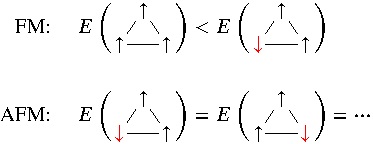
\includegraphics[width=0.5\linewidth]{ch2/frustrate.pdf}
\caption[Frustrated interactions in Ising model]{
Comparison between the non-frustrated FM and the frustrated AFM interactions for the Ising model on a triangle of three spins.
}
\label{fig:frustrate}
\end{figure}

On a triangular lattice of $N$ spins, the number of ground states $N_\text{GS}$ grows exponentially with $N$, which poses challenge for analytical and numerical methods to accurately evaluate the observables, or merely count the order of magnitude of $N_\text{GS}$. Besides the triangular lattice~\cite{li2015rare}, other kinds of frustrated lattices also appear in the modeling of materials, such as the kagome lattice~\cite{norman2016colloquium} and the pyrochlore (tetrahedral) lattice~\cite{harris1997geometrical}. The disordered ground states can lead to the spin liquid phase in the quantum description of these systems, which is an active topic of research.

At zero temperature, only the ground states contribute to the entropy $S = \ln N_\text{GS}$. In the thermodynamic limit $N \to \infty$, we assume $N_\text{GS} = A \rme^{c N}$, where $A$ and $c$ are coefficients to be determined. Then we have $\frac{S}{N} = \frac{\ln A}{N} + c$, which converges to $c$ as $N \to \infty$, and $c$ is known as the residual entropy~\cite{wannier1950antiferromagnetism, mambrini1999residual, vanderstraeten2018residual}. The existence of a non-zero residual entropy indicates the exponentially large number of degenerate ground states. For the relatively simple case of triangular Ising model, the analytical result has been derived~\cite{wannier1950antiferromagnetism, wannier1973antiferromagnetism}:
\begin{equation}
\lim_{L \to \infty} \lim_{\beta \to \infty} \frac{S}{N} = \frac{2}{\pi} \int_0^{\frac{\pi}{3}} \ln(2 \cos \omega) \dd \omega \approx 0.323.
\end{equation}
In addition, we mention that the boundary conditions of finite-sized systems can substantially affect the observables in the presence of frustration.

\subsection{Spin glass}
\label{sec:random-interactions}
\label{sec:sk}
\label{sec:ea}

Besides the geometrical frustration, another cause of disorder in Ising models is that the interactions $J_{i j}$ between the spins can be random. In this case, the Hamiltonian function is written as
\begin{equation}
H(\vs) = \sum_{i j} J_{i j} s_i s_j.
\label{eq:cl-ising-general}
\end{equation}
This kind of systems are known as spin glasses~\cite{fischer1993spin, nishimori2001statistical}, because of the analogy to the positional disorder in conventional amorphous glasses.

The Sherrington--Kirkpatrick (SK) model is defined by the fully connected Ising model in \cref{eq:cl-ising-general} with each interaction $J_{i j}$ sampled from a Gaussian distribution with zero mean and a variance of $\frac{1}{N}$.

The Edwards--Anderson (EA) model is defined by the Ising model in \cref{eq:cl-ising-general} with random interactions on a graph. The graph can be a 2D or 3D grid, as well as a random regular graph (RRG).

For the purpose of this thesis, we consider the EA model with binary interactions, where each $J_{i j}$ randomly takes $+1$ or $-1$ if there is an edge between $i$ and $j$ in the graph, and $0$ otherwise.

such as the quadratic unconstrained binary optimization (QUBO)~\cite{kochenberger2014unconstrained} and the maximum cut of weighted graphs~\cite{edwards1973some}.

Computational complexity of computing $Z$, so smart exact methods are not much better than brute force~\cite{barahona1982computational}









This means if we aim to exactly and provably find the ground state or its energy in the general case, then any smart algorithm is unlikely to be substantially faster than the brute-force enumeration. Therefore, we are further motivated to develop non-deterministic and heuristic approximation methods for this kind of problems.

\subsection{Associative memory}
\label{sec:hopfield}

The Hopfield model~\cite{hopfield1982neural, amit1985spin} is a model of associative memory. It is defined by the fully connected Ising model in \cref{eq:cl-ising-general} with the interactions
\begin{equation}
J_{i j} = -\frac{1}{N} \sum_{p = 1}^{n_\text{pat}} \xi^{(p)}_i \xi^{(p)}_j,
\label{eq:hopfield}
\end{equation}
where $\{\vxi^{(1)}, \vxi^{(2)}, \ldots, \vxi^{(n_\text{pat})}\}$ are some special spin configurations, known as the ``patterns'', and $n_\text{pat}$ is the number of patterns. We define the overlap between two configurations:
\begin{equation}
\ip{\vs}{\vs'} = \frac{1}{N} \sum_i s_i s'_i.
\label{eq:cl-overlap}
\end{equation}
The patterns need to be orthogonal:
\begin{equation}
\ip{\vxi^{(p)}}{\vxi^{(q)}} = 0, \quad \forall p, q.
\label{eq:cl-ortho}
\end{equation}
For any configuration $\vs$ and two orthogonal configurations $\vt_1$ and $\vt_2$, we have
\begin{equation}
|\ip{\vs}{\vt_1} + \ip{\vs}{\vt_2}| \le 1.
\end{equation}
The model has $2 n_\text{pat}$ degenerate ground states: $\vs_0 = \pm \vxi^{(p)}$, $H(\vs_0) = -N$. Therefore, we say the model ``memorizes'' the patterns.

Warshall ensemble

\subsection{Frustrated plaquette model}
\label{sec:fpm}

The 2D frustrated plaquette model (FPM) we consider in this work is defined as
\begin{align}
H(\vs) = &\phantom{{}+{}} J_1 \sum_{i, j = 1}^L s_{i, j} (s_{i + 1, j} + s_{i, j + 1}) \nonumber \\
&+ J_3 \sum_{i, j = 1}^L s_{i, j} (s_{i + 2, j} + s_{i, j + 2}) \nonumber \\
&+ K \sum_{i, j = 1}^L s_{i, j} \, s_{i + 1, j} \, s_{i, j + 1} \, s_{i + 1, j + 1},
\label{eq:fpm}
\end{align}

\begin{figure}[htb]
\centering
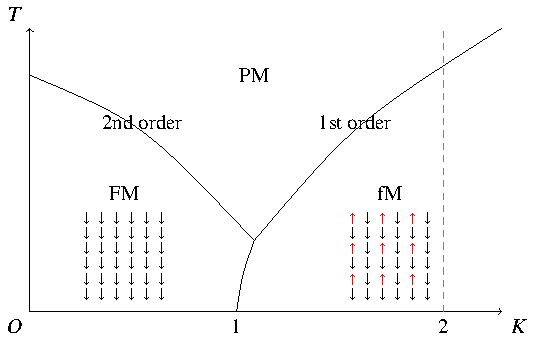
\includegraphics[width=0.7\linewidth]{ch2/fpm_phase.pdf}
\caption[Phase diagram of frustrated plaquette model (FPM)]{
Sketch of the phase diagram for the FPM with varying plaquette interaction strength $K$ and temperature $T$, at $J_1 = J_3 = -1$.
Examples of the ground state in the ferromagnetic (FM) and the ferrimagnetic (fM) phases are shown respectively.
The first-order phase transition at $K = 2$ is studied in Ref.~\cite{wu2021unbiased}, as indicated by the dashed vertical line.
This figure is reproduced from Fig.~3~(a) in Ref.~\cite{wu2021unbiased}.
}
\label{fig:fpm-phase}
\end{figure}

\section{Quantum systems}
\label{sec:qu-sys}

\subsection{Heisenberg model}

\begin{equation}
\hat{H} = J \sum_{\langle i, j \rangle} \hat{\vsi}_i \cdot \hat{\vsi}_j,
\label{eq:heis}
\end{equation}
where $\hat{\vsi}_i \cdot \hat{\vsi}_j = \hat{\sigma}^x_i \hat{\sigma}^x_j + \hat{\sigma}^y_i \hat{\sigma}^y_j + \hat{\sigma}^z_i \hat{\sigma}^z_j$ is the dot product of two 3D vectors of Pauli operators.

In the quantum case, we start from studying the ground state, or zero temperature properties of a system. The quantum state $\ket{\psi}$ of the system can be represented in the computational basis by
\begin{equation}
\ket{\psi} = \sum_\vs \psi(\vs) \ket{\vs},
\end{equation}
where $\vs$ is a vector of $N$ classical spin values, which is a possible outcome if we measure the quantum system along a chosen $z$ direction. The basis states $\{\ket{\vs}\}$ satisfy the orthonormal relation $\ip{\vs}{\vs'} = \delta_{\vs, \vs'}$, so we can project the state $\ket{\psi}$ onto a basis state $\ket{\vs}$ and obtain the corresponding wave function value $\psi(\vs) = \ip{\vs}{\psi}$, which is a complex number in general. Therefore, the state $\ket{\psi}$ is a complex vector in the Hilbert space of $2^N$ dimension. Moreover, it needs to satisfy the normalization condition $\ip{\psi}{\psi} = \sum_\vs |\psi(\vs)|^2 = 1$.

When the system is at the ground state, it is determined by the Hamiltonian operator $\hat{H}$ describing the system:
\begin{equation}
\ket{\psi_0} = \arg\min_{\ket{\psi}} \ev{\hat{H}}{\psi}.
\label{eq:gs}
\end{equation}
In contrast to the classical case, even if the quantum system is at the ground state and is non-degenerate, it can still be a superposition of exponentially many basis states.

Knowing the quantum state of the system, we can obtain the expectation value of any physical observable $\hat{O}$ by
\begin{equation}
\bar{O} = \ev{\hat{O}}{\psi} = \sum_{\vs, \vs'} \psi^*(\vs) O(\vs, \vs') \psi(\vs),
\label{eq:qu-obs}
\end{equation}
where $O(\vs, \vs') = \mel{\vs}{\hat{O}}{\vs'}$. Like the classical case, the summation in \cref{eq:qu-obs} also contains exponentially many terms and is intractable. Worse still, to exactly compute the ground state vector in \cref{eq:gs} in general, one needs the exact diagonalization (ED) of the $2^N \times 2^N$ Hamiltonian matrix, which takes even higher exponential time~\cite{weisse2008exact}. Therefore, we again need approximation methods to study the system in practice.

Stoquasticity, Marshall sign rule

QMA-complete~\cite{kempe2006complexity, troyer2005computational, oliveira2008complexity}

\subsection{Transverse-field Ising model (TFIM)}
\label{sec:qu-ising}

Tight banding~\cite{slater1954simplified}

Special case of anisotropic Heisenberg model~\cite{katsura1962statistical}

Phenomenological model with fictitious spins, such as the order-disorder transition of the ferroelectric crystal KH$_2$P0$_4$~\cite{de1963collective}.





simplest one to exhibit zero-temperature quantum phase transition driven by quantum fluctuations~\cite{sachdev2001quantum}


Ising ferromagnet

LiHOF$_4$~\cite{bitko1996quantum}

CoNb$_2$O$_6$~\cite{coldea2010quantum}

\begin{equation}
\hat{H} = J \sum_{\langle i, j \rangle} \hat{\sigma}^z_i \hat{\sigma}^z_j
+ \Gamma \sum_i \hat{\sigma}^x_i,
\label{eq:qu-ising}
\end{equation}
where the Pauli operators for spin-$\frac{1}{2}$ particles are represented by
\begin{equation}
\hat{\sigma}^x = \begin{pmatrix} 0 & 1 \\ 1 & 0 \end{pmatrix}, \quad
\hat{\sigma}^y = \begin{pmatrix} 0 & -i \\ i & 0 \end{pmatrix}, \quad
\hat{\sigma}^z = \begin{pmatrix} 1 & 0 \\ 0 & -1 \end{pmatrix}.
\end{equation}

We refer to Ref.~\cite{suzuki2012quantum} for the theoretical study of the phase transition in TFIM and its variants.

In 2D, $\Gamma_\text{c} \approx 3.04438(2)$~\cite{blote2002cluster}

\subsection{Quantum thermal state}

Beyond the ground state, the quantum system can be a mixed state characterized by a density matrix, and represented in the eigenbasis by
\begin{equation}
\hat{\rho} = \sum_i p_i \ket{\psi_i}\bra{\psi_i},
\end{equation}
where $\ket{\psi_i}$ is the $i$-th lowest eigenstate of the Hamiltonian, and $p_i$ is the corresponding probability of measuring this state. When the system is at the temperature $T$ in thermal equilibrium, $p_i$ is given by the Boltzmann distribution. Knowing the density matrix, we can obtain the expectation value of any physical observable $\hat{O}$ by
\begin{equation}
\bar{O} = \tr[\hat{O} \hat{\rho}].
\label{eq:dm-obs}
\end{equation}
The density matrix poses extra difficulties of computing both the states $\ket{\psi_i}$ and their probabilities $p_i$. In this thesis, we mainly focus on the ground state.
